% Dealerless Orca Ring-LPN proposal, v2.2 (2026-07-21).
% Restructured per advisor feedback on the 2026-06-10 draft:
%   1) problem overview  2) motivation (dealerless + GPU)
%   3) proposed design   4) experiment setup
% All "Figure 2" references to BCG+20 renamed to "BCG+20 generator";
% this document now contains its own figures.
% Numbers: measured values are regenerated from the current artifact CSVs;
% the distributed-keygen cost table is derived per DPF tree, including three
% scalar OLEs per tree and the bootstrap condition 3 c^2 t^2 < n.
\documentclass[11pt]{article}

\usepackage[margin=1in]{geometry}
\usepackage{amsmath,amssymb,amsthm}
\usepackage{booktabs}
\usepackage{array}
\usepackage{xcolor}
\usepackage{tikz}
\usetikzlibrary{positioning,arrows.meta,calc}
\usepackage{hyperref}

\hypersetup{
  colorlinks=true,
  linkcolor=blue!60!black,
  citecolor=blue!60!black,
  urlcolor=blue!60!black
}

\emergencystretch=1.5em % long unbreakable \texttt identifiers; avoid overfull lines

\newcommand{\Z}{\mathbb{Z}}
\newcommand{\Ring}{\mathcal{R}}
\newcommand{\ServerZero}{\mathsf{P}_0}
\newcommand{\ServerOne}{\mathsf{P}_1}
\newcommand{\bw}{\mathsf{bw}}
\newcommand{\modtwo}{\Z_{2^{\bw}}}
\newcommand{\Q}{Q}   % composite CRT modulus Q = p_0 p_1 (renamed from M to avoid clashing with the layer dimension M)

\title{Removing the Trusted Dealer from Orca's Linear Layers:\\
GPU-Accelerated Ring-LPN Preprocessing --- Status and Proposal (v2.2)}
\author{Ring-LPN / GPU-MPC project}
\date{2026-07-21 \quad (v2.2; corrects the D1 payload transcript and reports\\
the distributed key-generation protocol-logic host artifact of \S\ref{sec:m1proto})}

\begin{document}
\maketitle

\begin{abstract}
Orca performs two-party secure neural-network training and inference on GPUs,
but its preprocessing model requires a \emph{trusted dealer}: a third party
that generates all correlated randomness and could, if compromised, break the
privacy of every past computation at once. This document (1)~describes Orca's
current preprocessing architecture and the precise sense in which our existing
pipeline --- which already produces Orca's linear-layer keys from real
Ring-LPN correlation generators on GPUs, validated through Orca's unchanged
online code --- is \emph{not yet} dealerless; (2)~motivates removing the dealer
with GPU-accelerated pseudorandom correlation generators (PCGs), using
measured evidence for where the cost actually lives; (3)~proposes a concrete
design of five components (distributed key generation, PCG-sourced share
conversion, coin-tossed randomness, two-process deployment, and a security
parameter audit) and shows how they compose to remove every remaining trust
gap for the linear layers; and (4)~specifies the experimental setup: platform,
validation methodology, the measured baseline, and six milestone experiments,
each with a mechanical pass/fail gate. The first design component now has a
party-separated host \emph{protocol-logic and compatibility prototype} using
ideal OT/triple/OLE functionalities and the unchanged evaluator's explicitly
non-cryptographic correctness PRG. It functionally validates 2{,}432
two-party-generated DPF key pairs across six configurations up to the
production tree depth, includes edge cases and a corrupted-key control, and
models the distinguishing power of a sign opening removed in v2.2
(\S\ref{sec:m1proto}). This is evidence of executable correctness and
primitive accounting, not computational privacy or 128-bit security. All
performance claims are anchored in regenerated CSV artifacts; measured
numbers, derived numbers, and estimates are labelled as such throughout.
\end{abstract}

\section{Problem overview: Orca's preprocessing and its trusted dealer}
\label{sec:problem}

\subsection{Background: Orca in one page}
\label{sec:orca}

Orca~\cite{jawalkar2024orca} is a two-party secure computation (2PC) system
for neural-network training and inference, engineered around GPUs. Two servers
$\ServerZero$ and $\ServerOne$ hold additive secret shares of all inputs,
weights, and activations; neither learns anything beyond its own shares.
Like most practical 2PC systems, Orca splits work into an input-independent
\emph{preprocessing} (offline) phase that generates correlated randomness, and
a fast \emph{online} phase that consumes it:

\begin{itemize}
\item \textbf{Linear layers} (convolutions, fully-connected/FC layers) consume
  \emph{Beaver-triple--style matrix keys}: for a layer multiplying an
  $M{\times}K$ matrix by a $K{\times}N$ matrix, the parties need shares of
  random masks $A, B$ and of the product terms that make the masked
  multiplication identity work. Online, each party opens masked operands and
  runs the local computation implemented by \texttt{gpuMatmulBeaver}.
\item \textbf{Nonlinear layers} (ReLU, truncation) consume function secret
  sharing (FSS) keys --- distributed comparison functions (DCFs) --- with a
  different structure.
\end{itemize}

In stock Orca \emph{both} kinds of keys are produced by a \textbf{trusted
dealer}: a third machine that samples every mask, computes every correlated
value, and ships each party its key files (Figure~\ref{fig:dealer}).

\begin{figure}[t]
\centering
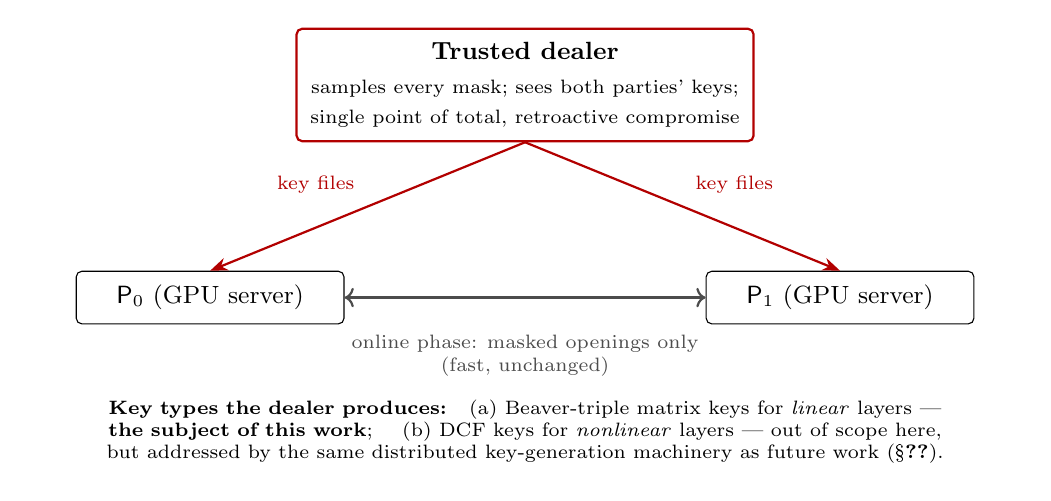
\begin{tikzpicture}[
  box/.style={draw, rounded corners=2pt, align=center, font=\small, inner sep=5pt},
  arr/.style={-{Stealth[length=2.2mm]}, thick},
  lbl/.style={font=\scriptsize, align=center}
]
\node[box, draw=red!70!black, thick, minimum width=52mm]
  (dealer) at (0,0) {\textbf{Trusted dealer}\\[1pt]
  \scriptsize samples every mask; sees both parties' keys;\\
  \scriptsize single point of total, retroactive compromise};
\node[box, minimum width=34mm] (p0) at (-40mm,-27mm) {$\ServerZero$ (GPU server)};
\node[box, minimum width=34mm] (p1) at (40mm,-27mm) {$\ServerOne$ (GPU server)};
\draw[arr, red!70!black] (dealer.south) -- (p0.north)
  node[lbl, midway, above left=0.5mm] {key files};
\draw[arr, red!70!black] (dealer.south) -- (p1.north)
  node[lbl, midway, above right=0.5mm] {key files};
\draw[arr, <->, black!70] (p0.east) -- (p1.west)
  node[lbl, midway, below=3.5mm] {online phase: masked openings only\\ (fast, unchanged)};
\node[lbl, text width=124mm] at (0,-44mm) {
  \textbf{Key types the dealer produces:}\quad
  (a) Beaver-triple matrix keys for \emph{linear} layers --- \textbf{the
  subject of this work}; \quad (b) DCF keys for \emph{nonlinear} layers ---
  out of scope here, but addressed by the same distributed key-generation
  machinery as future work (\S\ref{sec:threat}).};
\end{tikzpicture}
\caption{Orca's preprocessing today. The dealer is trusted with every secret
of the offline phase. This proposal removes it for the linear-layer keys;
the online phase is never modified.}
\label{fig:dealer}
\end{figure}

\subsection{Current status of our pipeline}
\label{sec:status}

Over the preceding milestones this project built, and validated on GPUs, a
preprocessing pipeline that produces Orca's FC-layer keys from \emph{Ring-LPN
pseudorandom correlation generators} rather than from a dealer's coin flips.
The pipeline (Figure~\ref{fig:pipeline}; components defined in
\S\ref{sec:design}) already works end-to-end with \emph{real} correlation
generators --- not idealized stand-ins --- at both supported modulus widths,
and its output keys are validated by the strongest referee available: Orca's
\emph{unchanged} online code reconstructs the correct products
(\S\ref{sec:baseline} gives the measured evidence).

\subsection{Why this is not yet dealerless}
\label{sec:gaps}

``The pipeline runs with real generators'' is not the same claim as ``the
dealer is gone.'' Five gaps remain; each is a precise, code-level statement,
and the design in \S\ref{sec:design} addresses them one for one.

\begin{description}
\item[G1 --- Centralized SPFSS key generation.] The correlation generator
  compresses each party's sparse noise into sums of distributed point
  functions (SPFSS; \S\ref{sec:motivation-pcg}). In our engine the function
  \texttt{build\_spfss\_keys()} currently reads \emph{both} parties' noise
  vectors and writes both key halves --- it is a dealer in miniature, marked
  as an oracle boundary in the source.
\item[G2 --- Dealer-supplied conversion correlations.] The pipeline computes
  over prime fields, Orca over $\modtwo$; the share conversion between them
  (\S\ref{sec:design-convert}) consumes edaBits, daBits and AND triples that a
  validated prototype currently takes from a labelled dealer block, and the
  end-to-end transcript still calls an exact conversion oracle.
\item[G3 --- Common-seed randomness.] Benchmarks derive \emph{both} parties'
  randomness from one \texttt{mt19937\_64} seed. A party knowing the seed can
  recompute the other party's secret noise outright, so this voids all
  security independently of every other parameter.
\item[G4 --- Unaudited security parameters.] The deployed noise parameters
  ($c{=}2$, $t{=}8$) are \emph{correctness} parameters for exercising the
  machinery. No concrete bit-security has been established, and our
  fully-splitting primes place us in the \emph{splittable} Ring-LPN regime,
  whose parameters must be derived independently (\S\ref{sec:design-params}).
\item[G5 --- Scope: nonlinear layers.] ReLU and truncation keys come from the
  same dealer via a different key type (DCF). They are explicitly out of
  scope for this proposal; \S\ref{sec:threat} states why the same machinery
  extends to them.
\end{description}

\paragraph{Contributions of this document.}
(1)~A gap analysis (G1--G5) separating what is verified from what is trusted;
(2)~a design of five components (D1--D5) that remove G1--G4, with the explicit
composition argument in Table~\ref{tab:composition};
(3)~a \emph{working host protocol-logic prototype of D1}, the distributed
key-generation component: the two-party protocol implemented party-separated
and functionally validated on 2{,}432 key pairs by the unchanged existing
evaluator, using ideal transport functionalities and a non-cryptographic
correctness PRG, with all primitive consumption measured
(\S\ref{sec:m1proto});
(4)~a re-derived, tree-accurate cost model for distributed key generation,
including a bootstrap self-sustainability condition ($3c^2t^2 < n$) that
couples the security audit to the key-generation design;
(5)~an experimental plan of six milestone experiments with mechanical
pass/fail gates, continuing the artifact discipline under which every number
in this document was produced.

\section{Motivation: why dealerless, and why on GPUs}
\label{sec:motivation}

\subsection{Why remove the dealer}
\label{sec:motivation-dealer}

The dealer is the single point of \emph{total, retroactive} compromise: it
holds every mask of every computation, so one breach --- or one subpoena, or
one insider --- retroactively breaks the privacy of everything the two parties
ever computed. The trust assumption is also operationally awkward: in many
two-party deployments (two mutually distrusting companies; a hospital and an
ML provider) no mutually trusted third machine exists, and dealer key material
for training runs is measured in gigabytes that must be generated, stored, and
shipped securely. Removing the dealer replaces an institutional assumption
with a cryptographic one.

\subsection{Why pseudorandom correlation generators, and which one}
\label{sec:motivation-pcg}

A training run consumes correlated randomness for billions of secure
multiplications; any protocol paying per-multiplication communication in the
offline phase is dead on arrival at that scale. Pseudorandom correlation
generators (PCGs)~\cite{boyle2019efficient,boyle2020ringlpn} restructure the
cost: the parties run one small interactive setup yielding short correlated
seeds, then each party \emph{locally} --- with zero communication,
``silently'' --- expands its seed into millions of correlated samples.

The atomic correlation we need is \emph{oblivious linear evaluation} (OLE):
$\ServerZero$ holds $u$, $\ServerOne$ holds $v$, and they obtain additive
shares of $u\cdot v$. Two OLEs make one Beaver triple; Beaver triples are
exactly what Orca's linear-layer keys package. The PCG we build on is the
ring-OLE generator of Boyle et al.~\cite{boyle2020ringlpn}, which we refer to
as the \textbf{BCG+20 generator}.\footnote{The construction is specified in
Figure~2 of~\cite{boyle2020ringlpn}; our codebase and earlier internal reports
call the implementation the ``Figure-2 engine'' after that figure number. The
present document uses ``BCG+20 generator'' to avoid referencing a figure that
does not appear in it.} In outline, over the negacyclic ring
$\Ring_p = \Z_p[X]/(X^n+1)$:

\begin{enumerate}
\item Each party $\sigma$ samples $c$ \emph{sparse} secret polynomials
  $e^{\sigma}_1,\dots,e^{\sigma}_c$ (only $t$ nonzero coefficients each). Its
  generator input is $x_\sigma = \sum_i a_i e^{\sigma}_i$ for public random
  $a_i$ --- pseudorandom under the Ring-LPN assumption
  (\S\ref{sec:design-params}).
\item The target product expands as
  $x_0 x_1 = \sum_{i,j} a_i a_j\,(e^0_i\, e^1_j)$: all secrecy concentrates in
  the $c^2$ products of sparse polynomials, and \emph{sparse times sparse
  stays sparse} --- each product has at most $t^2$ nonzeros, at positions that
  are \emph{sums} of the two parties' secret positions with values that are
  \emph{products} of their secret values.
\item Compact shares of such sparse vectors are exactly what sums of
  distributed point functions provide (SPFSS, built from DPF
  trees~\cite{boyle2015fss}): kilobyte-sized keys whose full-domain
  evaluations sum to the hidden sparse vector.
\item Each party locally evaluates its trees everywhere, multiplies by the
  public $a_i a_j$ (fast NTT polynomial arithmetic), and accumulates. Output:
  a \emph{ring OLE}, $z_0 + z_1 = x_0\, x_1$ in $\Ring_p$.
\end{enumerate}

\paragraph{Slot packing --- the amortization that makes this affordable.}
Our primes are chosen so that $X^n+1$ splits into $n$ linear factors mod $p$;
then the negacyclic number-theoretic transform (NTT) is a ring
\emph{isomorphism} $\Ring_p \to \Z_p^n$, and reading one ring OLE per
coordinate (``slot'') yields up to $n = 8{,}192$ \emph{independent scalar
OLEs} from a single ring-OLE expansion. Because the NTT is linear, each party
transforms its own shares locally. Measured consequence
(\S\ref{sec:baseline}): all linear-layer shapes in our suite consume exactly
$2L\lceil MKN/n\rceil$ ring OLEs ($L$ = number of CRT limbs, \S\ref{sec:notation})
--- e.g.\ \textbf{two} ring OLEs for an entire $16{\times}32{\times}16$ layer
at $\Q{=}p_0$, where the same layer would otherwise consume $16{,}384$
per-scalar OLE calls.

\subsection{Why GPUs}
\label{sec:motivation-gpu}

The motivation is empirical, not aesthetic. Profiling the expansion
(\S\ref{sec:baseline}) shows that \textbf{SPFSS full-domain evaluation ---
millions of independent AES/PRG invocations across thousands of DPF trees ---
dominates the cost} ($\sim$99\% at realistic noise weights; the NTT is under
1\%). That workload is embarrassingly parallel and exactly GPU-shaped, and it
is why our expansion runs in milliseconds on one GPU
(13.3\,ms at the smoke parameters; 61--881\,ms at $t{=}64$ depending on noise
regime). The proposed distributed key generation (\S\ref{sec:design-keygen})
preserves this shape: all trees advance \emph{level-synchronously}, so the
depth-14 tree walk has 14 sequential batches independent of how many
thousands of trees are in flight. This is not an end-to-end round count:
the input adder, correction-word openings, and two-stage payload
multiplication add dependency stages to be measured with M1's real transport.
Orca itself is GPU-resident; its randomness factory should live on the same
hardware, and our keys are written
byte-compatibly so Orca's GPU online path runs unmodified.

\subsection{Notation}
\label{sec:notation}

\begin{table}[ht]
\centering
\small
\begin{tabular}{ll}
\toprule
$M,K,N$ & linear-layer dimensions ($M{\times}K$ by $K{\times}N$ matmul)\\
$\bw$ & Orca's ring width; shares live in $\modtwo$ (bw $\le 32$ here)\\
$n$ & ring dimension; $\Ring_p = \Z_p[X]/(X^n+1)$, $n = 8192$\\
$p_0, p_1$ & NTT-friendly 62-bit primes $2^{62}-6\cdot2^{24}+1$,\ $2^{62}-7\cdot2^{24}+1$\\
$L$, $\Q$ & CRT limb count; composite modulus $\Q = p_0p_1$ ($L{=}1$: ``q64'', $\Q{=}p_0$; $L{=}2$: ``q128'')\\
$c, t$ & Ring-LPN noise parameters: $c$ sparse polynomials, $t$ nonzeros each\\
$\lambda$ & symmetric security parameter (AES/OT), $\lambda = 128$\\
\bottomrule
\end{tabular}
\end{table}

\section{Proposed design: a fully dealerless linear-layer pipeline on GPUs}
\label{sec:design}

\subsection{Design overview and principles}
\label{sec:design-overview}

Figure~\ref{fig:pipeline} shows the complete pipeline. Stages drawn solid are
implemented and gate-verified today; the two dashed stages are the oracle
boundaries G1 and G2, and the design components D1--D5 below replace them and
close G3--G4. Three principles carry over from how the existing artifact was
built:

\begin{enumerate}
\item \textbf{The online path is untouchable.} Keys are written
  byte-compatibly; Orca's online matmul (\texttt{gpuMatmulBeaver}) is both
  the consumer and the independent validation oracle. (With the integration flag off, baseline
  Orca is byte-identical --- verified.)
\item \textbf{Oracle boundaries are explicit.} Every idealized component is
  marked at the exact line in the source and named in every report; numbers
  produced with an oracle in the loop are never mixed with protocol-backed
  numbers in one table column.
\item \textbf{Every claim has a mechanical gate.} Components ship with
  suites that exit non-zero on any failure; one command re-validates the whole
  chain (\S\ref{sec:methodology}).
\end{enumerate}

\begin{figure}[t]
\centering
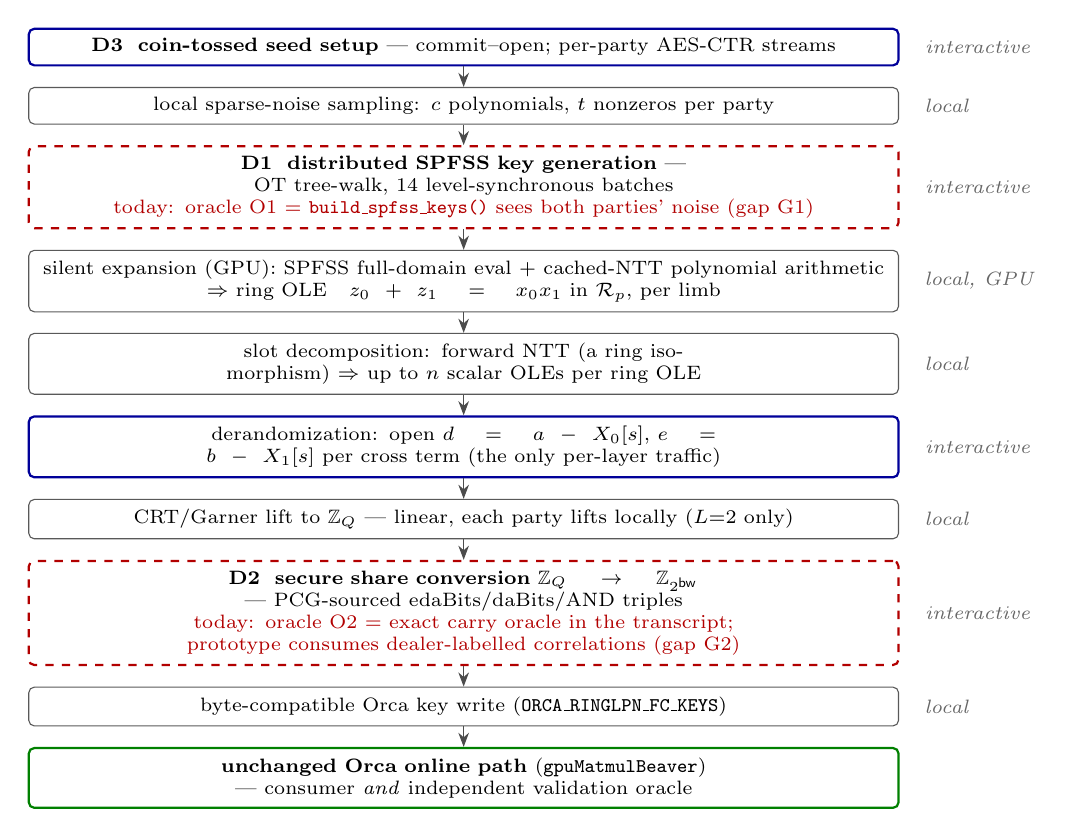
\begin{tikzpicture}[
  node distance=2.6mm,
  st/.style={draw, rounded corners=2pt, align=center, font=\scriptsize,
             inner sep=3.5pt, text width=108mm},
  loc/.style={st, draw=black!65},
  int/.style={st, draw=blue!60!black, thick},
  ora/.style={st, draw=red!70!black, thick, dashed},
  fin/.style={st, draw=green!50!black, thick},
  tag/.style={font=\scriptsize\itshape, text=black!60, anchor=west},
  arr/.style={-{Stealth[length=1.8mm]}, black!70}
]
\node[int] (coin) {\textbf{D3\ \ coin-tossed seed setup} --- commit--open; per-party AES-CTR streams};
\node[loc, below=of coin] (noise) {local sparse-noise sampling: $c$ polynomials, $t$ nonzeros per party};
\node[ora, below=of noise] (kg) {\textbf{D1\ \ distributed SPFSS key generation} --- OT tree-walk, 14 level-synchronous batches\\ \textcolor{red!70!black}{today: oracle O1 = \texttt{build\_spfss\_keys()} sees both parties' noise (gap G1)}};
\node[loc, below=of kg] (exp) {silent expansion (GPU): SPFSS full-domain eval $+$ cached-NTT polynomial arithmetic\\ $\Rightarrow$ ring OLE\quad $z_0+z_1 = x_0x_1$ in $\Ring_p$, per limb};
\node[loc, below=of exp] (slot) {slot decomposition: forward NTT (a ring isomorphism) $\Rightarrow$ up to $n$ scalar OLEs per ring OLE};
\node[int, below=of slot] (der) {derandomization: open $d = a - X_0[s]$,\ $e = b - X_1[s]$ per cross term (the only per-layer traffic)};
\node[loc, below=of der] (crt) {CRT/Garner lift to $\Z_\Q$ --- linear, each party lifts locally ($L{=}2$ only)};
\node[ora, below=of crt] (conv) {\textbf{D2\ \ secure share conversion} $\Z_\Q \to \modtwo$ --- PCG-sourced edaBits/daBits/AND triples\\ \textcolor{red!70!black}{today: oracle O2 = exact carry oracle in the transcript; prototype consumes dealer-labelled correlations (gap G2)}};
\node[loc, below=of conv] (wr) {byte-compatible Orca key write (\texttt{ORCA\_RINGLPN\_FC\_KEYS})};
\node[fin, below=of wr] (onl) {\textbf{unchanged Orca online path} (\texttt{gpuMatmulBeaver}) --- consumer \emph{and} independent validation oracle};
\foreach \a/\b in {coin/noise, noise/kg, kg/exp, exp/slot, slot/der, der/crt, crt/conv, conv/wr, wr/onl}
  \draw[arr] (\a) -- (\b);
\node[tag, right=2mm of coin.east] {interactive};
\node[tag, right=2mm of noise.east] {local};
\node[tag, right=2mm of kg.east] {interactive};
\node[tag, right=2mm of exp.east] {local, GPU};
\node[tag, right=2mm of slot.east] {local};
\node[tag, right=2mm of der.east] {interactive};
\node[tag, right=2mm of crt.east] {local};
\node[tag, right=2mm of conv.east] {interactive};
\node[tag, right=2mm of wr.east] {local};
\end{tikzpicture}
\caption{The proposed dealerless pipeline for one party (both parties run it
symmetrically; D4 deploys them as two processes over TCP). Solid boxes are
implemented and gate-verified today; dashed red boxes are the two oracle
boundaries (gaps G1, G2) that components D1 and D2 replace. Blue-framed
stages interact over the network; all others are local, and the heavy ones
run on the GPU.}
\label{fig:pipeline}
\end{figure}

\subsection{Setting and threat model}
\label{sec:threat}

Two computationally bounded parties; \textbf{semi-honest} (honest-but-curious)
adversary corrupting one of them. Assumptions: AES as PRG/PRF
($\lambda{=}128$); security of the OT-extension machinery
(Ferret-class~\cite{yang2020ferret}); hash-based commitments for coin tossing;
and the \emph{splittable} Ring-LPN assumption
(\S\ref{sec:design-params}). Out of scope, stated as claims discipline rather
than fine print: \textbf{malicious security} (consistency checks over OT
inputs and openings are known techniques and future work), and
\textbf{nonlinear layers} (their DCF keys are a second dealer axis; the D1
tree-walk machinery extends to them --- larger trees, different payload
groups, identical level-synchronous OT pattern --- as the natural follow-on
project). ``Dealerless Orca'' without the linear-layer qualifier is not
claimable at any milestone in this document.

\paragraph{Target model versus current D1 evidence.} The assumptions above
describe the \emph{target} pipeline: AES and real silent-OT/OLE transports.
The host artifact of \S\ref{sec:m1proto} instead uses counted ideal
OT/triple/OLE interfaces and the unchanged evaluator's splitmix64-based PRG,
which its source explicitly labels as non-cryptographic and correctness-only.
Accordingly, that artifact establishes protocol-logic compatibility, edge
correctness, and primitive counts; it does not establish computational
privacy or 128-bit security.

\subsection{D1: Distributed SPFSS key generation (removes G1)}
\label{sec:design-keygen}

\paragraph{What must be computed.} For each pair $(k,l)$ of noise nonzeros,
the parties must generate DPF keys for the point function with position
$\alpha = \mathrm{pos}^0_k + \mathrm{pos}^1_l$ (a value in $[0, 2n)$: products
of degree-$<n$ polynomials have unreduced degree up to $2n-2$; the negacyclic
fold $u[i] - u[i+n]$ is linear and applied locally after expansion) and
payload $\beta = \mathrm{val}^0_k \cdot \mathrm{val}^1_l \in \Z_p$. Observe
that the required sharing is \emph{already present in the problem}: $\alpha$
is additively shared (each party knows its own summand) and $\beta$ is
multiplicatively shared, with no extra protocol.

\paragraph{Protocol.} We adopt the Doerner--shelat two-party DPF key
generation~\cite{doerner2017floram} in the variant used by the PCG
literature~\cite{boyle2019efficient,boyle2020ringlpn}. The parties walk the
GGM tree level by level. Off the secret path the two parties' nodes are
identical, so XORing each party's aggregate PRG expansions leaves the on-path
contribution needed for that level's correction word. Selection by the
current secret-shared bit of $\alpha$ uses a 1-of-2 OT on
$\lambda$-bit strings. We keep control/tag bits separate from seed material,
following the original BGI-style construction and avoiding the insecure
seed-LSB optimization identified in the corrected full version of
BCG+20~\cite{boyle2020ringlpn}, \S5.2 and Remark~5.1.

For the arithmetic payload, let $A_b$ be party $b$'s signed leaf-seed
aggregate and $F_b$ its signed control-bit aggregate. A first scalar OLE
produces $\gamma_0+\gamma_1=\beta_0\beta_1=\beta$. Set
\[
d_0=\gamma_0-A_0,\quad d_1=\gamma_1-A_1,\qquad
s_0=F_0,\quad s_1=F_1,
\]
so $d_0+d_1=\beta-A_0-A_1$ and
$s_0+s_1=F_0+F_1\in\{+1,-1\}$. Two additional directional OLEs share
$d_0s_1$ and $s_0d_1$; adding those cross-term shares to the local products
$d_0s_0$ and $d_1s_1$ yields shares
$w_0+w_1=(d_0+d_1)(s_0+s_1)$. The parties open only this standard public
key material, $\mathit{finalCW}=w_0+w_1$; they never open the $d_b$, $s_b$,
or their sign. The predecessor transcript opened both $F_b$ values. Although
their sign is marginally independent of $\alpha$, conditioning on one
party's leaf control-bit vector makes it select the class containing
$\alpha$, so that opening was invalid.

The input bits of $\alpha$ come from a secure ripple adder
($\log(2n)-1$ Beaver bit triples). This is the concrete integration choice
for arithmetic position shares, not a claim of new ripple-adder research.
The known 1-OT-per-level walk optimization remains M1 engineering.

\paragraph{Prototype status (implemented; \S\ref{sec:m1proto}).} The
party-separated host implementation generates standard-format DPF keys from
shared $(\alpha,\beta)$ and passes full-domain validation by the
\emph{unchanged} existing evaluator on every tree tested: 2{,}432 key pairs,
both CRT primes, depths through $\log(2n)=14$. It uses ideal-functionality
OT, bit triples, and three scalar OLEs, plus the evaluator's non-cryptographic
correctness PRG; these are exactly why the executable is not evidence of
computational privacy. At depth 14 it measures 28 string OTs, 13 bit triples,
3 scalar OLEs, and 3{,}790 opened bits per tree. The old-sign regression
reconstructs the removed sign only in the omniscient harness and confirms
that it selects a proper leaf-control-bit class containing the true point;
this is a regression model of the old leak, not a privacy proof.

\paragraph{Bootstrapping (and why it is not circular).} Key generation
consumes three scalar OLEs per DPF tree; expansion produces $n$ slot OLEs per
ring OLE. The factory therefore feeds itself precisely when
\begin{equation}
3c^2 t^2 \;<\; n,
\label{eq:bootstrap}
\end{equation}
in which case the protocol runs in epochs --- a few output slots of each
epoch are reserved as the seed OLEs of the next, as
in~\cite{boyle2020ringlpn} --- and only epoch zero needs an external source
(a small fixed batch of OT-based Gilboa multiplications). At the smoke
parameters $(c,t,n)=(2,8,8192)$, key generation consumes 768 scalar-OLE
slots and the output/input surplus is $8192/768=10.67\times$.
Condition~\eqref{eq:bootstrap} \emph{couples the security audit to this
design}: if M5 (\S\ref{sec:milestones}) raises $t$ to $64$ at $n=8192$, then
$3c^2t^2=49{,}152>8{,}192$ and the ring dimension must grow with $t$ ---
consistent with the $n\ge 2^{16}$ parameter points in the literature.

\paragraph{GPU batching.} All trees of a generation batch advance
level-synchronously: the depth-14 tree walk has 14 sequential batched
AES/PRG expansions and OT selections, independent of tree count. The secure
ripple adder, correction-word openings, and two-stage payload multiplication
introduce additional dependency stages. End-to-end network rounds therefore
remain an M1 real-transport measurement, not a current result.

\paragraph{Cost model (per ring-OLE limb).} Each DPF tree of depth $d$ costs
$\lambda d$ correlated-OT instances; Ferret-class silent OT amortizes each
instance to roughly 1--8 bits of real traffic (implementation-maturity range;
M1 replaces this estimate with measurements). With uniform noise there are
$c^2t^2$ trees of depth $\log(2n) = 14$. With \emph{regular} noise (one
nonzero per width-$n/t$ bucket), the $t^2$ product points of each polynomial
pair fall on $2t-1$ predictable diagonals, so the same $c^2t^2$ trees shrink
to depth $\log(2n/t)$, grouped as $c^2(2t-1)$ SPFSS instances over the smaller
domain.\footnote{The 2026-06-10 draft priced the regular-noise row per SPFSS
\emph{instance} ($c^2(2t-1)$ units of depth 14), giving 107{,}520 OT
instances at $t{=}8$; the counts below are per DPF \emph{tree}, matching
\texttt{build\_spfss\_keys()}, and supersede it. Regular noise's decisive
advantage is expansion time and key size (measured $14\times$ and
$283{\to}233$\,kB at $t{=}64$), not OT volume.}

\begin{table}[ht]
\centering
\small
\begin{tabular}{lrrrrr}
\toprule
noise, $t$ ($c{=}2$) & DPF trees & depth & OT instances & scalar OLEs & est.\ silent-OT comm.\\
\midrule
uniform, $t{=}8$  & 256    & 14 & 458{,}752   & 768    & 0.06--0.46\,MB\\
regular, $t{=}8$  & 256    & 11 & 360{,}448   & 768    & 0.05--0.36\,MB\\
uniform, $t{=}64$ & 16{,}384 & 14 & 29{,}360{,}128 & 49{,}152 & 3.7--29\,MB\\
regular, $t{=}64$ & 16{,}384 & 8  & 16{,}777{,}216 & 49{,}152 & 2.1--17\,MB\\
\bottomrule
\end{tabular}
\caption{Distributed key-generation cost per ring-OLE limb (derived).
$n=8192$, $\lambda=128$; depth is $\log_2(2n)$ resp.\
$\log_2(2n/t)$. Scalar OLEs equal three times the tree count. The silent-OT
communication estimate excludes the still-unmeasured real OLE transport; M1
replaces both with measurements. The host prototype of
\S\ref{sec:m1proto} measures 2 string OTs per level (twice the table's
optimized 1-OT-per-level estimate), depth$-1$ bit triples, and three scalar
OLEs per tree.}
\label{tab:keygen}
\end{table}

\subsection{D2: PCG-sourced share conversion (removes G2)}
\label{sec:design-convert}

\paragraph{The problem.} The pipeline holds additive shares over $\Z_\Q$
(prime world, where NTTs exist); Orca needs shares over $\modtwo$ (hardware
world, where they do not). Reducing both shares mod $2^{\bw}$ is wrong
whenever the integer share-sum wrapped past $\Q$ --- and that \emph{wrap bit}
depends on both shares jointly, so computing it requires an actual secure
protocol.

\paragraph{The protocol (validated prototype).} With $S = z_0 + z_1 < 2\Q$
and $\ell = \lceil\log_2 2\Q\rceil$ ($\ell{=}63$ at q64, $125$ at q128):
(1)~mask-and-open $A = (z_0 + z_1 + R) \bmod 2^\ell$ using an
edaBit~\cite{escudero2020edabits} $R$ shared in both worlds ($A$ is uniform,
leaks nothing); (2)~a ripple adder over boolean shares recovers the bits of
$S = A - R$; (3)~a second adder computes the carry-out of $S + (2^\ell - \Q)$,
which \emph{is} the wrap bit $w = [S \ge \Q]$; (4)~a daBit converts $w$ to
arithmetic shares over $\modtwo$; (5)~each party locally corrects
$r_i = (z_i - \Q\, w_i) \bmod 2^{\bw}$. The prototype is bit-exact against
the all-seeing oracle on 8{,}512 conversions per configuration, and every
count in Table~\ref{tab:convert} is derivable: $2(\ell{-}1)$ AND triples (two
adders), $2\ell{-}1$ ripple rounds, $2\ell + 2\cdot\#\mathrm{AND} + 1$ opened
bits.

\paragraph{What D2 changes.} Two things. \emph{Sourcing:} AND triples come
from a binary PCG (the $\Z_2$ instantiation of our own pipeline, or
expand-accumulate codes~\cite{couteau2021silver}; Ferret~\cite{yang2020ferret}
yields them at $\sim$1 bit amortized), edaBits from random bit-shares by the
standard construction~\cite{escudero2020edabits} ($O(\ell)$ AND triples each,
one-time batch), daBits from the same batch. \emph{Depth:} the ripple
comparator becomes a parallel-prefix (Rabbit-style~\cite{makri2021rabbit})
comparison --- carries obey an associative generate/propagate rule, so all of
them come out of a $O(\log\ell)$-depth tree. Rounds are what network latency
multiplies; this swap is what makes the two-process deployment (D4) tolerable
over real wires.

\begin{table}[ht]
\centering
\small
\begin{tabular}{lrr}
\toprule
per $\modtwo$ output & q64 ($\ell{=}63$) & q128 ($\ell{=}125$)\\
\midrule
AND triples $=2(\ell{-}1)$ & 124 & 248\\
edaBit bits $=\ell$        & 63  & 125\\
daBits                     & 1   & 1\\
opened bits $=2\ell + 2\cdot\#\mathrm{AND} + 1$ & 375 & 747\\
AND rounds, ripple $=2\ell{-}1$ (measured today) & 125 & 249\\
AND rounds, prefix comparator (D2 target) & $\sim$7 & $\sim$8\\
\bottomrule
\end{tabular}
\caption{Measured conversion cost per output
(\texttt{secure\_convert\_prototype.csv}) with its closed-form derivations,
and the round-count target after the prefix-comparator swap. Triple and bit
counts grow by a small constant factor under the prefix comparator; rounds
drop from $O(\ell)$ to $O(\log\ell)$.}
\label{tab:convert}
\end{table}

\subsection{D3: Coin-tossed seeds and transcript hygiene (removes G3)}
\label{sec:design-seeds}

Replace every common \texttt{mt19937\_64} stream: \emph{shared, public}
randomness (the $a_i$, slot assignments) is derived from seeds fixed by
commit-then-open coin tossing over the existing \texttt{SigmaPeer} channel;
\emph{private} randomness comes from per-party AES-CTR streams; every derived
stream is domain-separated by the (layer, epoch, direction, limb) tuple
already used by \texttt{mixSeed}. This is bookkeeping, not research --- but it
is a hard precondition for any security claim, because a party that knows the
common seed can recompute the other party's sparse noise and simply read the
``hidden'' correlations off (zero bits of security regardless of $(n,c,t)$).

\subsection{D4: Two-process deployment (turns the transcript into a protocol)}
\label{sec:design-deploy}

Today's artifacts separate the parties logically within one process. D4
promotes them to two OS processes on two GPUs over the existing
\texttt{SigmaPeer} TCP layer (the same one Orca's two-party FC test uses).
The wire traffic is fully enumerable, which is the point: the derandomization
openings ($2\cdot 2\cdot MKN\cdot L$ field words per layer --- measured as
\texttt{opened\_words}, e.g.\ $32{,}768$ words $\approx 256$\,kB for the
full-capacity $16{\times}32{\times}16$ layer at q64), the per-level OT
messages of D1, and the conversion openings of D2 ($MN$ outputs
$\times$ Table~\ref{tab:convert}; note a layer has $MKN$ cross terms but only
$MN$ outputs, so conversion amortizes to $1/K$ of the cross-term work).

\subsection{D5: Security parameter audit (removes G4)}
\label{sec:design-params}

The assumption behind step 1 of \S\ref{sec:motivation-pcg} is
\textbf{Ring-LPN}: $(a, \sum_i a_i e_i + e_0)$ is pseudorandom for sparse
secret $e_i$. Our primes make $X^n+1$ split \emph{completely} --- that is what
buys slot packing --- but it also hands the attacker structure: a fully split
ring has CRT projections onto small quotients, giving decoding attacks
unavailable in the irreducible-ring variant. The honest hardness regime is
\emph{quasi-abelian decoding}~\cite{bombar2023quasiabelian}. D5 therefore
re-derives parameters rather than copying them: run standard
syndrome-decoding/ISD estimators against the splittable regime and pin
$(n, c, t, p_0, p_1)$ with estimator transcripts for $\ge 128$-bit security.
Representative literature points ($c{=}4$, $t$ in the dozens, $n \ge 2^{16}$
in BCG+20-style analyses) suggest $t$ will land well above the smoke value ---
which is why \S\ref{sec:baseline}'s $t{=}64$ measurements are quoted as the
realistic anchors, why regular noise (measured $14\times$ cheaper expansion)
is the default regime, and why condition~\eqref{eq:bootstrap} must be
re-checked at the audited parameters. Three engineering notes recorded with
reversal conditions: $v_2(p_0{-}1) = 25$ and $v_2(p_1{-}1) = 24$ leave
headroom to grow $n$ to $\sim 2^{23}$ without re-pinning primes; the 62-bit
prime class is what our Montgomery-based NTT supports (a faster external
library was rejected \emph{because} its Barrett reduction cannot run 62-bit
primes --- measured, documented); if D5 re-pins primes at $\le 60$ bits, that
NTT-backend decision re-opens.

\subsection{How the components compose to ``dealerless''}
\label{sec:design-composition}

\begin{table}[ht]
\centering
\small
\begin{tabular}{lll>{\raggedright\arraybackslash}p{4.6cm}}
\toprule
gap & removed by & verified at (gate) & claim unlocked\\
\midrule
G1 centralized keygen & D1 & M1, M2 & \emph{after M2:} keys from a two-party protocol whose only idealized part is the conversion\\
G2 conversion correlations & D2 & M3 & conversion protocol-backed end-to-end\\
G3 common-seed RNG & D3 & M4 (audited in review) & transcript hygiene preconditions met\\
(process separation) & D4 & M4 & \emph{after M4:} ``Orca FC preprocessing is dealerless (semi-honest, splittable Ring-LPN)''\\
G4 unaudited parameters & D5 & M5 & concrete $\ge$128-bit parameter claim\\
G5 nonlinear layers & out of scope & --- & never claimed here; D1 machinery extends (future work)\\
\bottomrule
\end{tabular}
\caption{Composition of the design: every gap of \S\ref{sec:gaps} maps to a
component and to the milestone experiment (\S\ref{sec:milestones}) whose
mechanical gate verifies its removal.}
\label{tab:composition}
\end{table}

\subsection{Per-layer cost model (worked example)}
\label{sec:design-cost}

For one FC layer $(M,K,N)$ at $L$ limbs, ring dimension $n$:
ring OLEs $= 2L\lceil MKN/n\rceil$;
derandomization traffic $= 2\cdot 2\cdot MKN\cdot L$ field words;
conversions $= MN$ (each per Table~\ref{tab:convert});
key-generation OT material per limb per Table~\ref{tab:keygen};
online phase unchanged (byte-compatible keys).
Worked example, $16{\times}32{\times}16$ at q64 ($L{=}1$, $\bw{=}16$):
$MKN = 8192$ cross terms per direction $\Rightarrow$ \textbf{2 ring OLEs};
$32{,}768$ opened words $\approx 256$\,kB; $MN = 256$ conversions
$\Rightarrow$ $31{,}744$ AND triples ($\sim$4\,kB of silent-OT traffic) and
256 daBits; keygen OT material $0.05$--$0.46$\,MB (Table~\ref{tab:keygen},
$t{=}8$). Every number above is either measured in the suite CSVs or derived
from a formula stated here.

\section{Experiment setup}
\label{sec:experiments}

\subsection{Platform and environment}
\label{sec:platform}

All measurements in this document were produced on one host: $4\times$ NVIDIA
RTX 5000 Ada (compute capability 8.9), CUDA 12.6, Linux. Builds run either on
the host (\texttt{nvcc} on \texttt{PATH}) or in the project's
\texttt{orca-dev} container; two-party tests run as two processes pinned to
distinct GPUs via \texttt{CUDA\_VISIBLE\_DEVICES}, communicating over TCP
loopback through Orca's \texttt{SigmaPeer} layer. The GPU NTT backend is a
cheddar-derived merged-stage kernel family (signed Montgomery arithmetic;
q32/q64/q128-CRT; negacyclic) with the Hadamard product adaptively fused into
the inverse-NTT load and forward NTTs of fixed public vectors cached across
expansion iterations.

\subsection{Validation methodology}
\label{sec:methodology}

Three rules, applied to every artifact. (1)~\emph{Independent oracles}: fast
implementations are validated against separately written references --- the
GPU NTT against a host reference (\texttt{host\_polymul\_reference}), the
generator's internals against host suites (135/57/36 host validation cases),
the end-to-end pipeline against Orca's \emph{unchanged} online code
reconstructing the correct product. (2)~\emph{Party-separation discipline}:
transcript artifacts compute each party's view in separated state; any read
across the boundary is an explicitly named oracle. (3)~\emph{Mechanical
gates}: every artifact ships source + build script + run script + CSV/MD/log;
suites exit non-zero on any failure; one command re-validates every claim in
this document ($\sim$15 min on one GPU):
\begin{center}
\texttt{RUN\_GPU\_SMOKE=1 REQUIRE\_GPU\_SMOKE=1 scripts/run\_paper\_checkpoint\_smoke.sh}
\end{center}
which must print \texttt{ALL GATES PASS}.

\subsection{Verified baseline (measured, 2026-06-10 artifacts)}
\label{sec:baseline}

\paragraph{End-to-end real-generator transcript.} The flagship
suite\footnote{Artifact \texttt{bench\_orca\_fc\_real\_ole\_transcript}; per-case
results in Table~\ref{tab:suite}'s source CSV.} (9 cases) drives the full
pipeline of Figure~\ref{fig:pipeline} with the real BCG+20 generator ---
oracles only at O1/O2 --- and validates through unchanged
\texttt{gpuMatmulBeaver} at q64 ($\bw \le 16$) and q128 ($\bw = 32$, two CRT
limbs, per-party Garner lift), under uniform and regular noise: 9/9 pass.

\begin{table}[ht]
\centering
\small
\begin{tabular}{lrrrrr}
\toprule
case & ring OLEs & ideal-OLE equiv. & slots used & opened $\Z_p$ words & contract\\
\midrule
q64, $16{\times}32{\times}16$, $\bw{=}16$ & 2 & 16{,}384 & 8{,}192 & 32{,}768 & pass\\
q128, $16{\times}16{\times}16$, $\bw{=}32$ & 4 & 8{,}192 & 4{,}096 & 32{,}768 & pass\\
\bottomrule
\end{tabular}
\caption{Representative rows of the flagship suite
(\texttt{orca\_fc\_real\_ole\_\allowbreak transcript\_\allowbreak
transcript\_\allowbreak suite.csv}). ``Ideal-OLE equiv.''\ is the number of
per-scalar OLE calls the same layer consumed before slot packing.}
\label{tab:suite}
\end{table}

\paragraph{Distributed key-generation protocol-logic prototype
(corrected 2026-07-21).}
\label{sec:m1proto}
The artifact\footnote{\texttt{test\_distributed\_dpf\_keygen}; per-case
results in \texttt{distributed\_dpf\_keygen\_prototype.csv}.} implements the
two-party key-generation protocol of \S\ref{sec:design-keygen}
party-separated on the host. Cross-party values flow only through counted
ideal functionalities (1-of-2 string OT, Beaver bit triples, and three
scalar OLEs) or explicit openings. It emits the standard existing
\texttt{spfss\_host::DPFKey} format, consumed by the untouched
\texttt{spfss\_host::dpfEvalAll}. That evaluator uses a splitmix64
correctness PRG explicitly labelled non-cryptographic; the artifact is
therefore a protocol-logic and compatibility prototype, not a secure/private
implementation.

The suite (Table~\ref{tab:m1proto}) generates 2{,}432 key pairs across six
configurations, tree depths 4--14, and both CRT primes. Every pair
full-domain-evaluates to $\beta\cdot[x{=}\alpha]$. In every configuration,
the first two trees deterministically cover $\alpha=0$ and
$\alpha=2^L-2$, factors $1$ and $p-1$, and resulting payloads $p-1$ and
$1$; the remaining trees use random nonzero payload factors. A centralized
reference passes through the same evaluator, while a corrupted correction
word fails. The field
\texttt{old\_sign\_opening\_leak\_control=yes} records that the omniscient
regression model reconstructed the removed sign and observed a proper
party-0 leaf-control-bit class containing the true point. This demonstrates
the old transcript's distinguishing power; it is not a privacy proof. The
gate is wired into the repository's one-command re-validation
(\S\ref{sec:methodology}).

\begin{table}[ht]
\centering
\small
\begin{tabular}{lrrrrrrr}
\toprule
prime & depth & trees & pass & string OTs & bit triples & OLEs & opened bits\\
\midrule
$p_0$ & 4  & 512 & 512/512 & 8  & 3  & 3 & 1{,}170\\
$p_0$ & 8  & 512 & 512/512 & 16 & 7  & 3 & 2{,}218\\
$p_0$ & 11 & 384 & 384/384 & 22 & 10 & 3 & 3{,}004\\
$p_0$ & 14 & 256 & 256/256 & 28 & 13 & 3 & 3{,}790\\
$p_1$ & 14 & 256 & 256/256 & 28 & 13 & 3 & 3{,}790\\
$p_1$ & 8  & 512 & 512/512 & 16 & 7  & 3 & 2{,}218\\
\bottomrule
\end{tabular}
\caption{Distributed key-generation protocol-logic prototype: regenerated
results (\texttt{distributed\_\allowbreak dpf\_\allowbreak keygen\_\allowbreak
prototype.csv}). Per-tree counts
match $2\cdot$depth string OTs, depth$-1$ bit triples, three scalar OLEs, and
$2(\mathrm{depth}-1)+260\cdot\mathrm{depth}+124$ opened bits. The depth-14
host timing is approximately 1.8\,ms per tree, single-threaded and including
validation; timings are approximate run observations, not transport
measurements. Table~\ref{tab:m1proto} proves functional compatibility, edge
correctness, and primitive accounting, not computational privacy or
128-bit security.}
\label{tab:m1proto}
\end{table}

\paragraph{Performance anchors.}
Ring-OLE expansion ($n{=}8192$, $c{=}2$): 13.3\,ms (q64) and 26.8\,ms (q128)
at the $t{=}8$ smoke point; at $t{=}64$: 881\,ms uniform vs.\ \textbf{61\,ms
regular} ($14\times$), with pair-key bytes 283\,kB vs.\ 233\,kB. SPFSS
full-domain evaluation dominates ($\sim$99\%); the NTT is under 1\% ---
measured directly, and confirmed by the fact that a 2--8\% NTT-side
improvement left expansion time unchanged. Conversion prototype: bit-exact on
8{,}512 conversions per configuration at the costs of
Table~\ref{tab:convert}. Byte-compatibility: with the integration flag off,
baseline Orca output is byte-identical (verified through the real two-party
FC test).

\subsection{Planned experiments: six milestones with mechanical gates}
\label{sec:milestones}

\begin{figure}[ht]
\centering
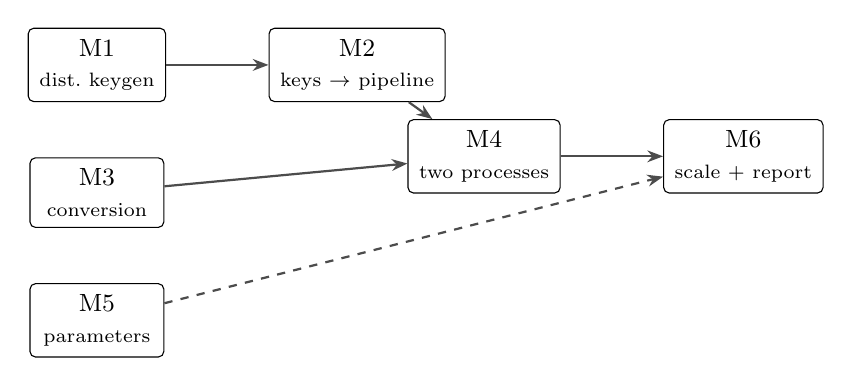
\begin{tikzpicture}[
  m/.style={draw, rounded corners=2pt, font=\small, inner sep=4pt, minimum width=17mm, align=center},
  arr/.style={-{Stealth[length=2mm]}, thick, black!70}
]
\node[m] (m1) {M1\\ \scriptsize dist.\ keygen};
\node[m, below=7mm of m1] (m3) {M3\\ \scriptsize conversion};
\node[m, below=7mm of m3] (m5) {M5\\ \scriptsize parameters};
\node[m, right=13mm of m1] (m2) {M2\\ \scriptsize keys $\to$ pipeline};
\node[m, right=13mm of $(m2.east)!0.5!(m3.east)$, yshift=-3.5mm] (m4) {M4\\ \scriptsize two processes};
\node[m, right=13mm of m4] (m6) {M6\\ \scriptsize scale + report};
\draw[arr] (m1) -- (m2);
\draw[arr] (m2) -- (m4);
\draw[arr] (m3) -- (m4);
\draw[arr] (m4) -- (m6);
\draw[arr, dashed] (m5) -- (m6);
\end{tikzpicture}
\caption{Milestone dependencies. M1, M3, M5 are mutually independent and can
proceed in parallel; M5 (dashed) gates only the security column of M6's
report.}
\label{fig:milestones}
\end{figure}

\begin{description}
\item[M1 --- Distributed DPF keygen prototype (GPU-batched).]
  Implements D1. \emph{Gate:} for random additively shared $\alpha$ and
  multiplicatively shared $\beta$, the generated key halves full-domain
  evaluate to the point function for every tree in a batch of $\ge256$; the
  GPU key format is byte-identical so \texttt{gpuDpfZpFullEvalSum} runs
  unmodified. \emph{Metrics:} real OT/OLE bytes, wall-clock per batch, and
  end-to-end network rounds. \emph{Status:} the host artifact of
  \S\ref{sec:m1proto} discharges only the protocol-logic and host-format
  functional slice (batches $\ge256$, depth 14, unchanged host evaluator).
  M1 still requires AES/CSPRNG evaluation, real silent-OT/OLE transport, GPU
  level-synchronous batching, byte-identical GPU keys, and measured bytes and
  rounds.
\item[M2 --- Real-generator transcript driven end-to-end by M1 keys.]
  \emph{Gate:} the existing 9/9 suite passes with
  \texttt{build\_spfss\_keys()} replaced by the two-party protocol; the only
  remaining oracle is the conversion. (Because the key format is unchanged,
  any new failure localizes to the new keygen.)
\item[M3 --- PCG-sourced conversion + prefix comparator.] Implements D2.
  \emph{Gate:} the conversion suite (\texttt{test\_secure\_convert}) passes
  bit-exact with correlations consumed from the binary PCG instead of the
  dealer block;
  measured round count drops to $O(\log\ell)$ (Table~\ref{tab:convert}).
\item[M4 --- Two-process deployment over TCP.] Implements D4 (with D3's
  coin-tossed seeds). \emph{Gate:} the full pipeline (M1 keygen $\to$ expand
  $\to$ derandomize $\to$ convert $\to$ key write) runs as two OS processes on
  two GPUs; the \texttt{gpuMatmulBeaver} contract passes; communication
  measured and reported per layer.
\item[M5 --- Security parameter memo.] Implements D5. \emph{Gate:} pinned
  $(n, c, t)$ with estimator evidence for $\ge 128$-bit splittable Ring-LPN
  security; headline tables regenerated at the pinned parameters; bootstrap
  condition~\eqref{eq:bootstrap} re-checked.
\item[M6 --- Scale and report.] \emph{Gate:} dealerless preprocessing for the
  FC layers of one Orca model, with a table comparing trusted-dealer versus
  dealerless preprocessing on time, communication, and key bytes --- with no
  mixing of oracle-backed and protocol-backed numbers in a single column.
\end{description}

\subsection{Reporting and claims discipline}
\label{sec:claims}

The claims ladder is part of the experimental design. \emph{Already claimable
(from \S\ref{sec:m1proto})}: ``the distributed key-generation protocol logic
is implemented party-separated and functionally validated by the unchanged
evaluator, using ideal OT/triple/OLE functionalities and a non-cryptographic
correctness PRG.'' This is deliberately not a claim of computational
privacy, 128-bit security, M1 completion, GPU byte compatibility, real
transports, or two-process isolation. \emph{After M2}: ``linear-layer Beaver
keys are generated by a two-party protocol whose only idealized component is
the share conversion.'' \emph{After M4}: ``Orca FC preprocessing is
dealerless (semi-honest, splittable Ring-LPN).'' \emph{Never claimable within
this proposal's scope}: malicious security; any concrete security level
before M5; ``dealerless Orca'' without the linear-layer qualifier. Every
measured table in the final report carries the regenerating command;
oracle-backed and protocol-backed numbers never share a column; decisions
carry written reversal conditions (e.g., the NTT-backend choice re-opens if
M5 re-pins primes below 61 bits).

\section{Related work}
\label{sec:related}

Orca~\cite{jawalkar2024orca} defines the host system: FSS-based 2PC ML on
GPUs with a dealer-based preprocessing model. Beaver's
technique~\cite{beaver1991} underlies the linear-layer keys. The PCG line ---
silent OT extension and PCGs from LPN~\cite{boyle2019efficient}, ring-OLE PCGs
from Ring-LPN~\cite{boyle2020ringlpn} --- provides our correlation generator;
Ferret~\cite{yang2020ferret} and Silver~\cite{couteau2021silver} provide
practical silent OT/VOLE for D1's tree-walk material and D2's binary triples.
DPFs originate in the FSS line~\cite{boyle2015fss}; distributed DPF key
generation without a dealer is due to Doerner and
shelat~\cite{doerner2017floram}. Mixed arithmetic--binary conversions use
edaBits/daBits~\cite{escudero2020edabits} and Rabbit-style
comparison~\cite{makri2021rabbit}. The concrete hardness of our fully-split
(splittable / quasi-abelian) Ring-LPN regime is analyzed by Bombar et
al.~\cite{bombar2023quasiabelian}.

\section{Summary}
\label{sec:summary}

Orca's linear-layer preprocessing already runs, measured and gate-verified,
from real Ring-LPN correlation generators on GPUs --- with exactly two
idealized components left in that pipeline (key generation and share
conversion) and three hygiene/audit obligations (seeds, deployment,
parameters). D1 now has a host protocol-logic and compatibility prototype:
2{,}432 standard key pairs pass the unchanged evaluator with edge, reference,
corruption, and old-leak regression controls, using ideal transport
functionalities and a non-cryptographic correctness PRG. This is research
progress suitable for evaluating the M1 design, not evidence that M1 or
computational privacy is complete. D1--D5 remove the remaining boundaries
along M1--M6. Only after that ladder completes is ``dealerless Orca
linear-layer preprocessing (semi-honest, splittable Ring-LPN)'' an honest,
reproducible claim.

\begin{thebibliography}{9}
\bibitem{jawalkar2024orca}
N.~Jawalkar, K.~Gupta, A.~Basu, N.~Chandran, D.~Gupta, R.~Sharma.
\emph{Orca: FSS-based Secure Training and Inference with GPUs}.
IEEE S\&P 2024.
\bibitem{beaver1991}
D.~Beaver. \emph{Efficient Multiparty Protocols Using Circuit Randomization}.
CRYPTO 1991.
\bibitem{boyle2015fss}
E.~Boyle, N.~Gilboa, Y.~Ishai. \emph{Function Secret Sharing}.
EUROCRYPT 2015.
\bibitem{boyle2019efficient}
E.~Boyle, G.~Couteau, N.~Gilboa, Y.~Ishai, L.~Kohl, P.~Scholl.
\emph{Efficient Pseudorandom Correlation Generators: Silent OT Extension and
More}. CRYPTO 2019.
\bibitem{boyle2020ringlpn}
E.~Boyle, G.~Couteau, N.~Gilboa, Y.~Ishai, L.~Kohl, P.~Scholl.
\emph{Efficient Pseudorandom Correlation Generators from Ring-LPN}.
CRYPTO 2020; corrected full version, IACR ePrint 2022/1035 (2022),
\S5.2 and Remark~5.1.
\bibitem{doerner2017floram}
J.~Doerner, a.~shelat. \emph{Scaling ORAM for Secure Computation}.
CCS 2017.
\bibitem{yang2020ferret}
K.~Yang, C.~Weng, X.~Lan, J.~Zhang, X.~Wang.
\emph{Ferret: Fast Extension for Correlated OT with Small Communication}.
CCS 2020.
\bibitem{couteau2021silver}
G.~Couteau, P.~Rindal, S.~Raghuraman.
\emph{Silver: Silent VOLE and Oblivious Transfer from Hardness of Decoding
Structured LDPC Codes}. CRYPTO 2021.
\bibitem{escudero2020edabits}
D.~Escudero, S.~Ghosh, M.~Keller, R.~Rachuri, P.~Scholl.
\emph{Improved Primitives for MPC over Mixed Arithmetic-Binary Circuits}.
CRYPTO 2020.
\bibitem{makri2021rabbit}
E.~Makri, D.~Rotaru, F.~Vercauteren, S.~Wagh.
\emph{Rabbit: Efficient Comparison for Secure Multi-Party Computation}.
FC 2021.
\bibitem{bombar2023quasiabelian}
M.~Bombar, G.~Couteau, A.~Couvreur, C.~Ducros.
\emph{Correlated Pseudorandomness from the Hardness of Quasi-Abelian
Decoding}. CRYPTO 2023.
\end{thebibliography}

\end{document}
